\subsection{Simulation Results}

Fig.~\ref{fig:ser16} and Fig.~\ref{fig:ser32} compare the symbol error
rate (SER) performance of different detectors under 64-QAM modulation
for the $16\times16$ and $32\times32$ MIMO settings, respectively. In
both cases, the linear MMSE detector gives the highest SER because it
cannot sufficiently suppress the residual inter-stream interference.
OAMP improves upon MMSE through iterative decoupling, while EP provides
a stronger classical baseline by refining the approximate posterior
distribution during the iterations.

For the $16\times16$ system in Fig.~\ref{fig:ser16}, the learning-aided
detectors consistently outperform the classical baselines as the SNR
increases. GEPNet and GCEPNet reduce the SER by incorporating
correlation information into the EP-based neural refinement. DEPNet
achieves the best performance over the whole SNR range, and its
advantage becomes more evident in the high-SNR region, where more
accurate posterior tracking directly translates into lower error rates.

Fig.~\ref{fig:ser32} further shows that the same trend remains valid in
the larger $32\times32$ system. Although the stronger inter-stream
coupling makes detection more challenging, DEPNet still outperforms
GEPNet and GCEPNet at every tested SNR point. In particular, DEPNet
achieves about $1$\,dB gain over GCEPNet at SER\,$=10^{-4}$ for
\mbox{$N_t\!=\!N_r\!=\!32$}. This consistent improvement stems from
DEPNet's ability to track the evolving EP belief. The sparse coupling
graph, content-adaptive attention, and cross-attention work together to
exploit posterior information that static graph filtering cannot
capture, yielding progressively more accurate symbol estimates as EP
converges.

\begin{figure}[t]
    \centering
    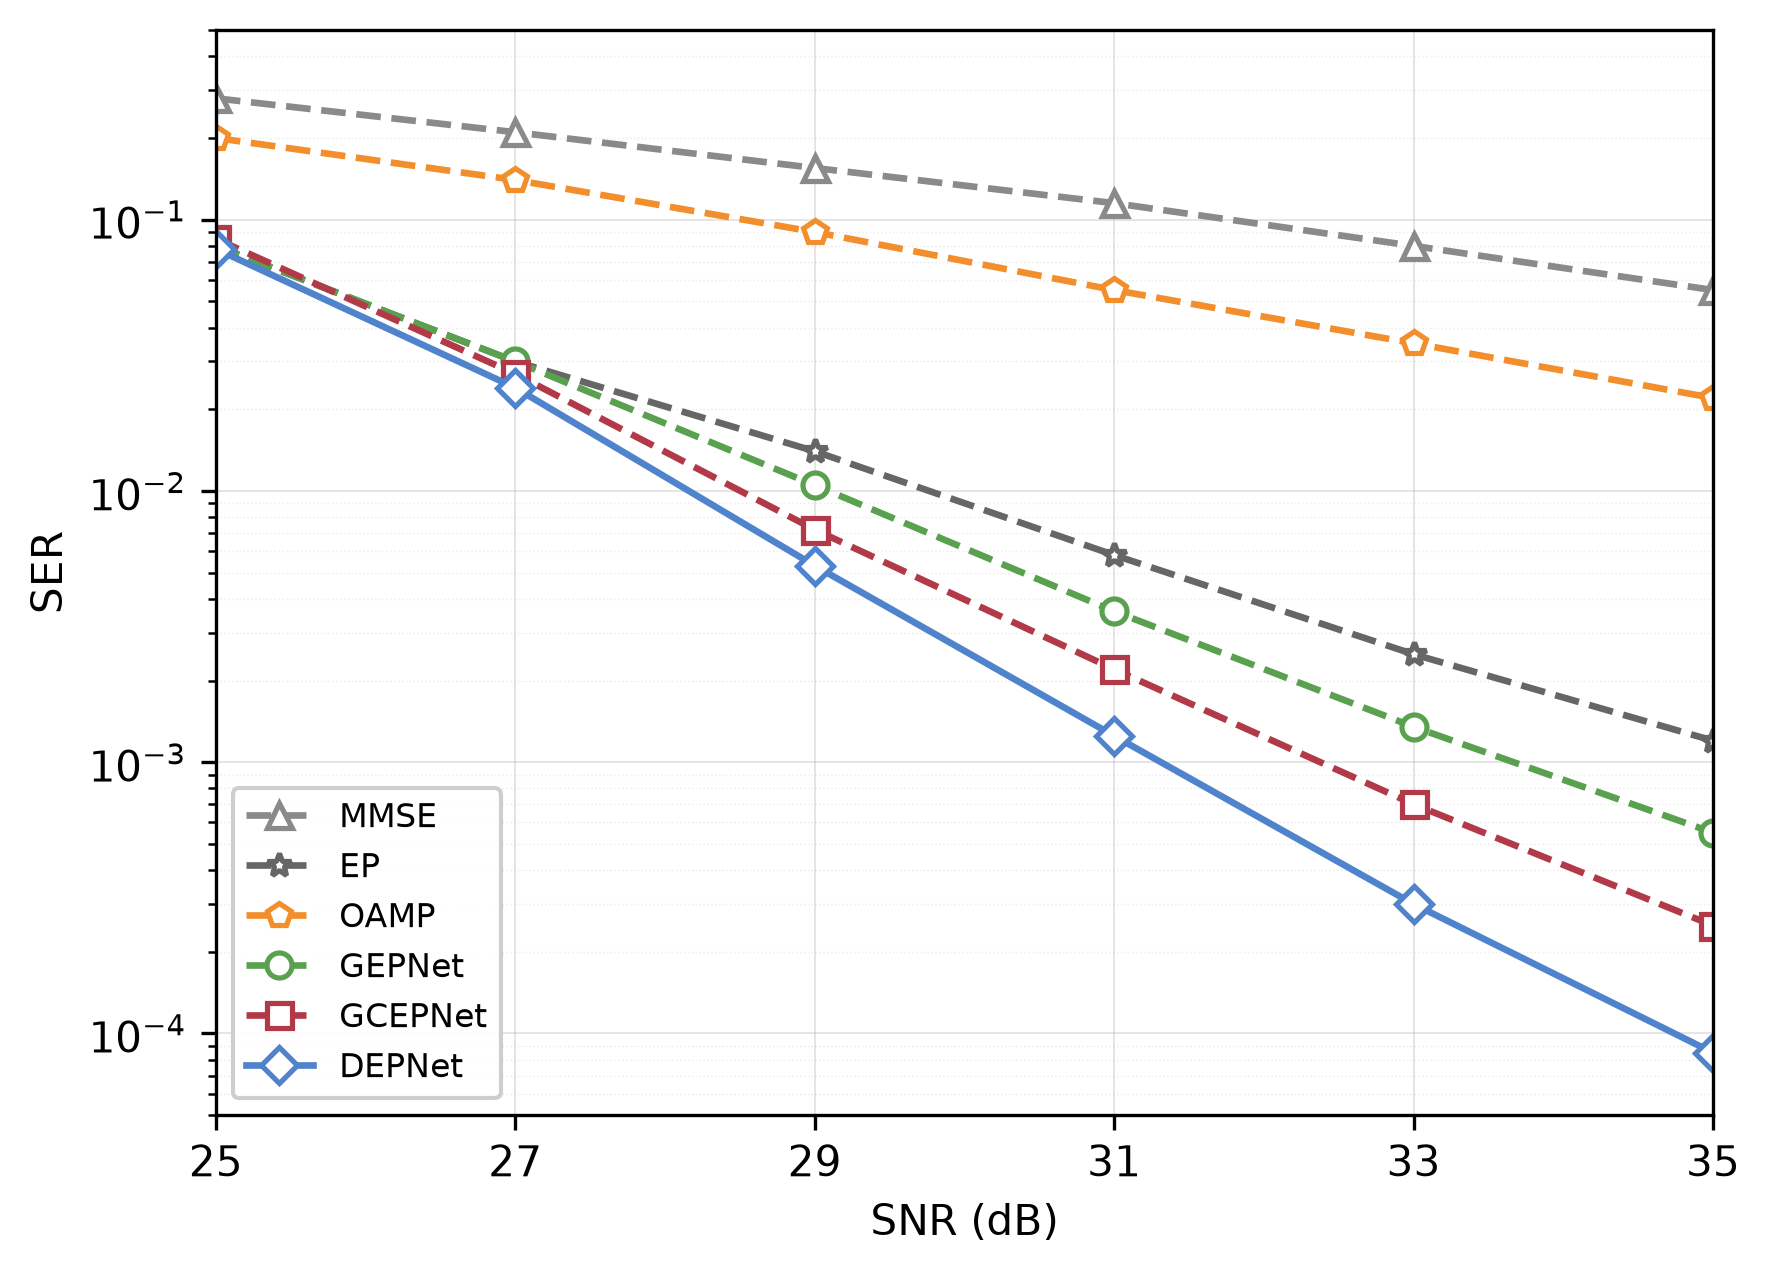
\includegraphics[width=0.9\columnwidth]{figs/ser_comparison_16x16_64QAM.png}
    \caption{The SER performance comparison for the $16\times16$ 64-QAM system.}
    \label{fig:ser16}
\end{figure}

\begin{figure}[t]
    \centering
    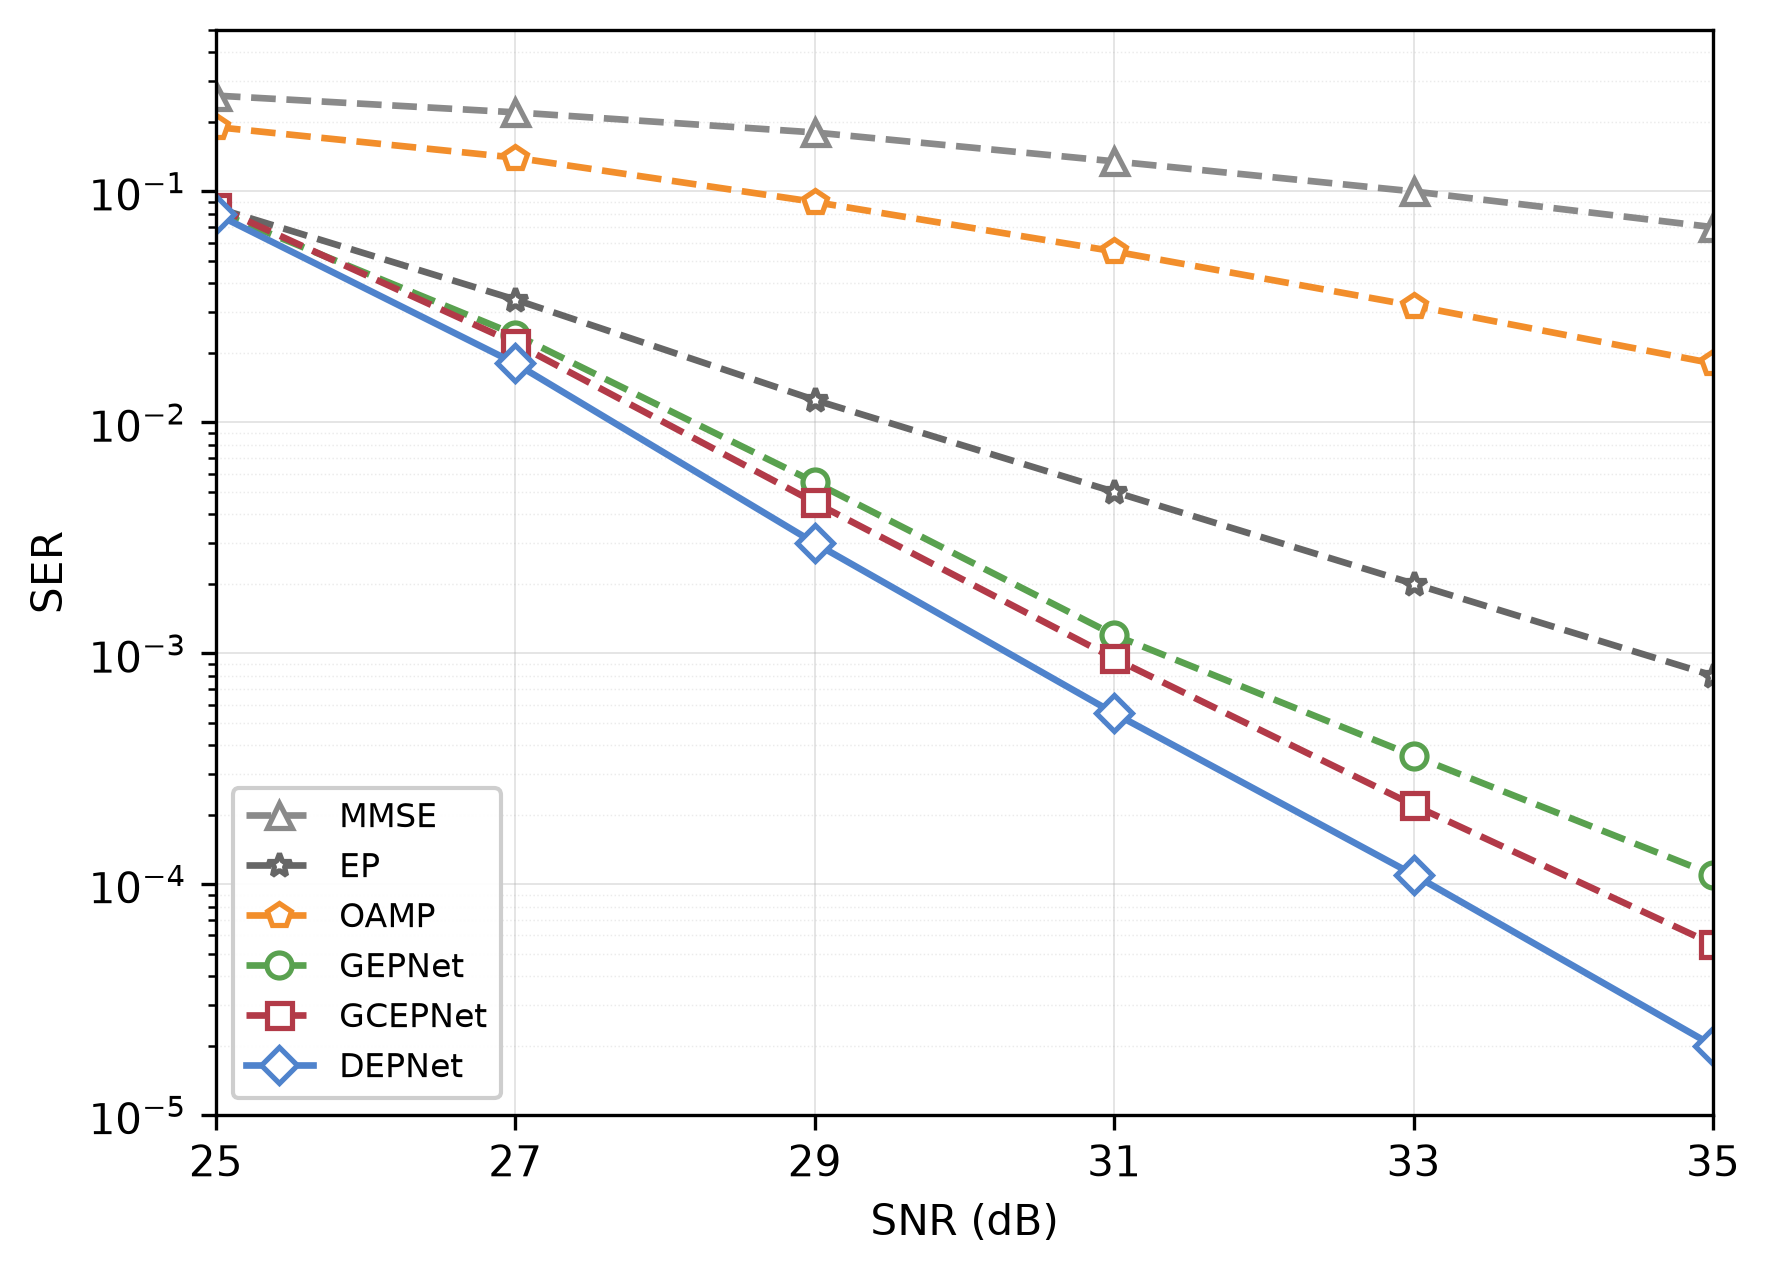
\includegraphics[width=0.9\columnwidth]{figs/ser_comparison_32x32_64QAM.png}
    \caption{The SER performance comparison for the $32\times32$ 64-QAM system.}
    \label{fig:ser32}
\end{figure}
